\chapter{Calcul littéral} \label{N3}

\vfill

\begin{figure}[h]
   \centering
      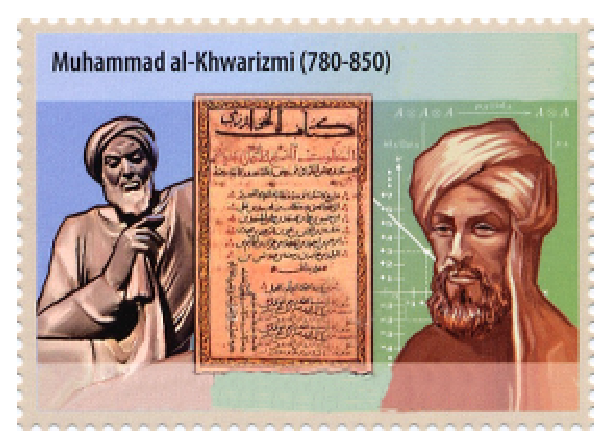
\includegraphics[height=7cm]{Nombres_et_calculs/Images/N3_intro_Alkhwarizmi}
   \caption{Timbre Al-Khwarizmi}
\end{figure}

\vfill

\begin{prerequis}[Un peu d'histoire]
   Le mathématicien perse {\bf Muhammad bin Musa Al-Khawarizmi} ($\approx$780-850), est à l'origine des mots \textit{algorithme}, issu de son nom et \textit{algèbre}, issu d'une méthode et du titre de l'un de ses ouvrages. Son apport en mathématiques est tel qu'il est surnommé \og le père de l'algèbre \fg, avec {\bf Diophante d'Alexandrie}, dont il reprendra les travaux. En effet, il est le premier à répertorier de façon systématique des méthodes de résolution d'équations en les classant dans son ouvrage {\it Kitab al-mukhtasar fi hisab al-jabr wa'l muqabala} qui signifie {\it Livre sur la science de la transposition et de la réduction}. L'acte de naissance officiel de l'Algèbre est la publication de ce livre, dédié au calife {\bf al-Ma'moun}. 
\end{prerequis}


\cours %%%%%%%%%%%%%%%%%%%%%%%

\section{Calculs avec des puissances entières} %%% 1

\begin{definition}[Notation]
   $$\underbrace{a\times a\times\cdots\times a}_{\hbox{$n$ facteurs}} =a^n \qquad ; \qquad \underbrace{10\times10\times\cdots\times10}_{\hbox{$n$ facteurs}} =10^n$$
\end{definition}

\begin{exemple*1}
   $(-5)^3 =(-5)\times(-5)\times(-5) =-125$ \hfill $10^4 =10\times10\times10\times10 =10\,000$.
\end{exemple*1}

\smallskip

Par convention, on pose \quad $a^0=1$ \quad pour tout nombre $a$ non nul.

\begin{propriete}[Règles de calcul]
   Pour tout réel $a$ non nul et pour tous entiers relatifs $m$ et $n$, on a les propriétés suivantes : \\
   Produit de puissances : $a^m\times a^n =a^{m+n}$ \hfill Puissance de puissance : $\left(a^m\right)^n=a^{m\times n}$ \\ [1mm] 
   Inverse d'une puissance : $a^{-n}=\dfrac{1}{a^n}$ \hfill Fraction de puissances : $\dfrac{a^m}{a^n} =a^{m-n}$ 
\end{propriete}

\begin{exemple*1}
   $2^3\times2^4 = 2^{3+4} =2^7$ \hfill $2^{-3} =\dfrac{1}{2^3}$ \hfill $\dfrac{10^5}{10^2} =10^{5-2} =10^3$ \hfill $\left(4^2\right)^3 =4^{2\times3} =4^6$.
\end{exemple*1}

\smallskip

Lorsque les valeurs d'une grandeur sont très grandes ou très petites dans l'unité choisie, il est commun d'utiliser un préfixe dans le nom de l'unité : 

\begin{Ctableau}{\linewidth}{11}{c}
   \hline
   Puissance & $10^9$ & $10^6$ & $10^3$ & $10^2$ & $10^{1}$ & $10^{-1}$ & $10^{-2}$ & $10^{-3}$ & $10^{-6}$ & $10^{-9}$ \\
   \hline
   Préfixe & giga & méga & kilo & hecto & déca & déci & centi & milli & micro & nano \\
   \hline
   Symbole & G & M & k & h & da & d & c & m & $\mu$ & n \\
   \hline
\end{Ctableau}

 
\section{Calculs avec des radicaux} %%% 2

\begin{definition}[Racine carrée]
   Soit $a$ un nombre positif. On appelle \textbf{racine carrée} du nombre $a$ le seul nombre positif dont le carr\'e est $a$. On note ce nombre $\sqrt{a}$.
\end{definition}

\begin{remarque}
   pour tout nombre réel $a$, on a $\sqrt{a^2} =|a|$.
\end{remarque}

Il est utile de connaître les premiers carrés parfaits afin de simplifier, ou calculer plus rapidement une racine carrée :
\begin{center}
   \begin{Ctableau}{0.8\linewidth}{13}{c}
      \hline
      $a$ & 1 & 2 & 3 & 4 & 5 & 6 & 7 & 8 & 9 & 10 & 11 & 12 \\
      \hline
      $a^2$ & 1 & 4 & 9 & 16 & 25 & 36 & 49 & 64 & 81 & 100 & 121 & 144 \\
      \hline
   \end{Ctableau}
\end{center}

\begin{propriete}[Opérations élémentaires]
   Pour tous nombres positifs $a$ et $b$, avec $b$ non nul s'il est placé au dénominateur : \vspace*{-2mm}
   $$\sqrt{a \times b} =\sqrt{a} \times \sqrt{b} \qquad ; \qquad \sqrt{\dfrac{a}{b}} = \dfrac{\sqrt{a}}{\sqrt{b}}$$ \vspace*{-8mm}
   $$\attention \qquad \sqrt{a+b} \neq \sqrt{a} + \sqrt{b} \qquad ; \qquad \sqrt{a - b} \neq\sqrt{a} - \sqrt{b}$$
\end{propriete}

\begin{exemple*1}
$\sqrt{72} = \sqrt{36 \times 2} = \sqrt{36} \times \sqrt{2} = 6\sqrt2 \qquad ; \qquad \sqrt{\dfrac{25}{121}} = \dfrac{\sqrt{25}}{\sqrt{121}} = \dfrac{5}{11}$. \\ [1mm]
   $\sqrt{ 64 + 36} = \sqrt{100} = \sqrt{10^{2}} = 10$ \qquad mais \qquad $\sqrt{64} + \sqrt{36} = \sqrt{8^{2}} + \sqrt{6^{2}} = 8 + 6 = 14$.
\end{exemple*1}


\section{Transformation d'écritures littérales} %%% 3


\subsection{Développement}  % A

\begin{definition}[Dévélopper]
   \textbf{Développer}, c'est passer d'un produit à une somme (on enlève les parenthèses).
\end{definition}

\begin{propriete}[Distributivité]
   Distributivité simple : \qquad $k\times(a+b)=k\times a+k\times b =ka+kb$ \\
   Distributivité double : \qquad $(a+b)(c+d)=a\times c+a\times d+b\times c+b\times d =ac+ad+bc+bd$
\end{propriete}

\begin{exemple*1}
    $3\times(2x-1) =3\times(2x)+3\times(-1) =6x-3$. \\
    $(x+2)(x-3) =x\times x+x\times(-3)+2\times x+2\times(-3) =x^2-3x+2x-6$.
\end{exemple*1}

\begin{definition}[Simplifier]
   \textbf{Simplifier} une expression, c'est écrire une expression équivalente plus simple en regroupant les termes de même type.
\end{definition}
   
\begin{exemple*1}
   $(x+2)(x-3) =x^2-3x+2x-6 =x^2-x-6$. \\
   $3x+5t+2x-2t=3x+2x+5t-2t=5x+3t$.
\end{exemple*1}


\subsection{Factorisation} % B

\begin{definition}[Factoriser]
   \textbf{Factoriser}, c'est passer d'une somme à un produit (on ajoute des parenthèses).
\end{definition}

\begin{exemple*1}
   $5x+40=\underline{5}\times x+\underline{5}\times8 =\underline{5}\times(x+8) =5(x+8)$. \\
   Factoriser $3x+5y$ est impossible car il n'y a aucun facteur en commun dans les deux termes.
\end{exemple*1}

\begin{propriete}[Identités remarquables]
   Pour distribuer ou factoriser, on peut utiliser les identités remarquables suivantes : \vspace*{-2mm}
   \begin{center}
      $(a+b)^2 =a^2+2ab+b^2$ \\
      $(a-b)^2 =a^2-2ab+b^2$ \\
      $(a+b)(a-b) =a^2-b^2$
   \end{center}
\end{propriete}

\begin{exemple*1}
   $(2x-3)^2 =(2x)^2-2\times2x\times3+3^2 =4x^2-12x+9$. \\
   $9x^2-16 =(3x)^2-4^2 =(3x+4)(3x-4)$.
\end{exemple*1}


\subsection{Valeur absolue et intervalle}  % C

\begin{propriete}[Écriture d'un intervalle]
   Lorsqu'un intervalle s'écrit sous la forme $[\,a-r\,;\,a+r\,]$, avec $r>0$, on dit que l'intervalle a pour centre $a$ et pour rayon $r$ et on peut écrire : \\
   \hspace*{4cm} $x\in[a-r\,;\,a+r]\iff|x-a|\leq r$ \smallskip
\end{propriete}

\begin{center}
   \begin{pspicture}(-3,0)(3,0.7)
      \psline{->}(-3,0)(3,0)
      \rput(-2,0){|}
      \rput(-2,-0.4){$a-r$}
      \rput(0,0){|}
      \rput(0,-0.4){$a$}
      \rput(2,0){|}
      \rput(2,-0.4){$a+r$}
      \psline[linecolor=A1]{<->}(-2,0.3)(0,0.3)
      \rput(-1,0.6){$r$}
      \psline[linecolor=A1]{<->}(2,0.3)(0,0.3)
      \rput(1,0.6){$r$}
   \end{pspicture}
\end{center}


\section{Résolution d'équations} %%% 4

\subsection{Règles générales} % A

\begin{definition}[Équation]
   Une \textbf{équation} est une égalité entre deux expressions où apparaissent des {\bf inconnues} désignées par des lettres. \textbf{Résoudre} l'équation, c'est trouver toutes les valeurs possibles pour l'inconnue. \smallskip
\end{definition}

\begin{propriete}[Addition d'un terme et Multiplication par un scalaire]
   \begin{itemize}
      \item Dans une équation, on ne change pas les solutions en ajoutant ou en soustrayant un même nombre à chaque membre.
      \item Dans une équation, on  ne change pas les solutions en multipliant ou en divisant chaque membre par un même nombre non nul. \\ \vspace*{-8mm}
   \end{itemize}
\end{propriete}


\subsection{Équation du type \bm{$ax+b =0$}} % B

\begin{propriete}[Solution]
   L'équation $ax+b =0$ avec $a\neq0$ a une seule solution : $x =-b\div a=-\dfrac{b}{a}.$
\end{propriete}

\begin{preuve}
   On soustrait $b$ de chaque côté de l'égalité : $ax+b-b =0-b$ c'est à dire $ax =-b$, \\
   on divise chaque membre par $a$, on obtient l'équation $\cancel ax\div \cancel a=-b\div a$, c'est à dire $x=-b\div a$.
\end{preuve}

\begin{exemple*1}
   $4x-8 =0 \iff 4x-\cancel8\,\textcolor{A1}{+\,\cancel8} =0\,\textcolor{A1}{+\,8}$ \hfill On ajoute 8 de chaque côté de l'égalité \\
   \hspace*{3.2cm} $\iff 4x =8$ \\
   \hspace*{3.2cm} $\iff \cancel4x\,\textcolor{A1}{\div\,\cancel4} =8\,\textcolor{A1}{\div\,4}$ \hfill On divise par 4 de chaque côté de l'égalité \\
   \hspace*{3.2cm} $\iff x =2$.  
\end{exemple*1}

\subsection{Équation du type \bm{$ax+b =cx+d$}} % C

\begin{propriete}[Résolution]
   Pour résoudre une équation du type $ax+b=cx+d$, on regroupe les termes \og en $x$ \fg{} d'un même côté de l'égalité et les nombres de l'autre côté.
\end{propriete}

\begin{exemple*1}
   Résolution l'équation $5x+4=2x-5$ : \\
   \begin{tabular}{p{11cm}p{4cm}}
      on regroupe les $x$ à gauche par soustraction de $2x$ à gauche et à droite & $5x+4\,\textcolor{A1}{-\,2x}=\cancel{2x}-5\,\textcolor{A1}{-\,\cancel{2x}}$ \\
      on réduit les expressions obtenues & $3x+4=-5$ \\
      on regroupe les nombres à droite par soustraction de $4$ à gauche et à droite & $3x+\cancel4\,\textcolor{A1}{-\,\cancel4}=-5\,\textcolor{A1}{-\,4}$ \\
      on réduit les expressions obtenues & $3x=-9$ \\
      on divise chaque membre de l'équation par $3$ & $\cancel3x\,\textcolor{A1}{\div\,\cancel3} =(-9)\,\textcolor{A1}{\div\,3}$ \\
      on réduit les expressions obtenues & $x=-3$ \\ [-5mm]
   \end{tabular}
\end{exemple*1}


\subsection{Équation-produit} % D

\begin{propriete}[Produit de facteurs nul]
   Un produit de facteurs est nul si, et seulement si, l'un des facteurs est nul. \\
   \hspace*{4cm} $A\times B =0 \iff A =0 \text{ ou } B =0$ \smallskip
\end{propriete}

\begin{exemple*1}
   Résolution de l'équation $(x-4)(2x+5)=0$. \\
   Un produit de facteurs est nul si, et seulement si, l'un au moins de ses facteurs est nul : \\ [1mm]
   $\begin{array}{rcll}
      (x-4)(2x+5) = 0 & \iff & x-4 = 0 \text{ ou } 2x+5 = 0 \\
      & \iff & x- \cancel4 \textcolor{A1}{\,+\,\cancel4} = 0 \textcolor{A1}{\,+\,4} \text{ ou } 2x+\cancel5 \textcolor{A1}{\,- \,\cancel5\,} =0 \textcolor{A1}{\,- \,5} \\
      & \iff & x = 4 \text{ ou } 2x =-5 \\
      & \iff & x = 4 \text{ ou } x = -\dfrac52 \\
   \end{array}$ \\
   Les solutions de l'équation $(x-4)(2x+5) = 0\,$ sont $-\dfrac52$ et $4$. 
\end{exemple*1}


%\subsection{Résolution de problèmes} % D
%\begin{methode}[Résolution d'un problème nécessitant une équation]
%Certains problèmes peuvent être résolus grâce à la résolution d'une équation. Plusieurs étapes sont nécessaires :
%\begin{enumerate}
%   \item choix de l'inconnue ;
%   \item mise en équation du problème ;
%   \item résolution de l'équation ;
%   \item interprétation du résultat et éventuellement vérification du résultat.
%\end{enumerate}
%
%\exercice
%   Trouver trois nombres consécutifs dont la somme est $153$.
%   
%\correction
%   \ \\ [-10mm]
%   \begin{itemize}
%      \item \textbf{Choix de l'inconnue :} on note $n$ le premier de ces trois, le deuxième nombre est alors $n+1$ et le troisième $n+2$.
%      \item \textbf{Mise en équation :} $(n)+(n+1)+(n+2)=153$, \\
%      c'est à dire : $n+n+1+n+2=153$, soit $3n+3=153$.
%      \item \textbf{Résolution de l'équation :} $3n+3-3=153-3$, \\
%      soit $3n=150$, donc $n=150\div3= 50$.
%      \item \textbf{Interprétation du résultat :} les trois nombres recherchés sont 50, 51 et 52. Vérification : $50+51+52=153$.
%   \end{itemize}
%\end{methode}


\section{Résolution d'une inéquation} %%% 5

\begin{propriete}[Ordre d'une inéquation]
   \begin{itemize}
      \item L'ordre est {\bf conservé} lorsqu'on ajoute (ou soustrait) un même nombre aux deux membres d'une inégalité ou lorsqu'on multiplie (ou divise) les deux membres d'une inégalité par un même nombre strictement positif.
      \item L'ordre est {\bf inversé} lorsqu'on multiplie (ou divise) les deux membres d'une inégalité par un même nombre strictement négatif. \\ [-8mm]
   \end{itemize}
\end{propriete}

\begin{exemple*1}
   \begin{itemize}
      \item Si $x+7 < 4$ alors $x+\cancel7 \textcolor{A1}{\,-\,\cancel7\,} < 4 \textcolor{A1}{\,-\,7\,}$ donc $x < -3$ \quad ({\it soustraction d'un nombre}). \rule[-5pt]{0pt}{5pt}
      \item Si $ 6x > 24$ alors $\dfrac{\cancel6x}{\textcolor{A1}{\cancel6}} > \dfrac{24}{\textcolor{A1}{6}}$ donc $x > 4$ \quad ({\it division par un nombre positif}). \rule[-10pt]{0pt}{10pt}
      \item Si $ -5x < 35$ alors $\dfrac{-\cancel5x}{\textcolor{A1}{-\cancel5}} > \dfrac{35}{\textcolor{A1}{-5}}$ donc $x > -7$ \quad ({\it division par un nombre négatif}). \\ [-6mm]
   \end{itemize}
\end{exemple*1}

\medskip

Résoudre une inéquation revient à déterminer toutes les valeurs possibles de l'inconnue telle que l'inégalité soit vraie. On obtient un intervalle, qui peut être réduit à un point ou aucun point.

\begin{exemple*1}
  Résoudre l'inéquation : $3x - 2 > 5x + 8$. \\
   $3x - 2 > 5x + 8
   \begin{array}[t]{lccc}      
      \iff & 3x - 2 \textcolor{A1}{\,-\,5x\,} & > & \cancel{5x} + 8 \textcolor{A1}{\,-\,\cancel{5x}\,} \\
      \iff & -2x - 2 & > & 8 \\
      \iff & -2x - \cancel2 \textcolor{A1}{\,+\,\cancel2\,} & > & 8 \textcolor{A1}{\,+\,2\,} \\
      \iff & -2x & > & 10 \\ [1mm]
      \iff & \dfrac{-\cancel2x}{\textcolor{A1}{-\cancel2}} & < & \dfrac{10}{\textcolor{A1}{-2}} \\ [2mm]
      \iff & x & < & -5 \\
   \end{array}$ \\ [2mm]
   Les solutions de l'inéquation $3x - 2 > 5x + 8$ sont les nombres $x$ strictement inférieurs à $-5$. \\
   On peut écrire $\mathcal{S} =]\,-\infty\,;\,-5\,[$.
\end{exemple*1}
 

%%%%%%%%%%%%%%%%%%%%%%%%%
%%%%%%%%%%%%%%%%%%%%%%%%%
\activites

\begin{activite}[Groupement 1 - Exercice 3 : résolution de problème, équation]
   \ \\ [-16mm]
   \begin{QCM}
      Un enseignant d’une classe de CM2 a proposé ce problème à ses élèves. \\ [1mm]
\fbox{\parbox{16cm}{\it Dans un bocal, un enfant a des billes vertes, des billes rouges et des billes bleues. Il a 4 fois plus de billes rouges que de billes vertes et il a 3 billes vertes de plus que de billes bleues. En tout il a 51 billes. \\
Combien a-t-il de billes de chaque couleur ?}} \\ [1mm]
{\scriptsize D'après un problème du Guide pour enseigner la résolution de problèmes au cours moyen, Ministère de l'éducation nationale, 2021.}
\begin{enumerate}
   \item Voici la réponse proposée par Samira, une élève de la classe de CM2 :
      \begin{center}
         \psset{unit=0.75}
         \begin{pspicture}(1,0.25)(16,7.25)
            \psframe(0,0.25)(16,7.25)
            \psframe(3,5.25)(3.5,4.75)
            \psarc(6.75,4.75){0.25}{-90}{0}
            \psline(7,4.75)(7,5.5)
            \psarc(7.25,5.5){0.25}{90}{180}
            \psarc(7.25,6){0.25}{180}{-90}
            \psline(7,6)(7,6.75)
            \psarc(6.75,6.75){0.25}{0}{90}
            \psset{fillstyle=solid,fillcolor=lightgray}
            \rput[l](0.5,0.75){Il y a 8 billes vertes, 32 billes rouges et 11 billes bleues, ça fait bien 51 billes.}
            \rput[l](2,1.5){$8+3 =11$}
            \psframe(2,2)(3,2.5)
            \rput[l](3.25,2.25){$=8$ \hspace{1.5cm} $4\times8 =32$}
            \rput[l](2,3){6}
            \psframe(2.5,2.75)(3.5,3.25)
            \rput[l](3.75,3){$=48$}
            \rput[l](2,3.75){$51-3 =48$}
            \rput[l](0.3,5){Bleues}
            \psframe(2,4.75)(3,5.25)
            \rput[l](3.15,5){3}
            \rput[l](0.3,5.75){Rouges}
            \psframe(2,5.5)(3,6) \psframe(3,5.5)(4,6) \psframe(4,5.5)(5,6) \psframe(5,5.5)(6,6)
            \rput[l](0.3,6.5){Vertes}
            \psframe(2,6.25)(3,6.75)
            \rput[l](7.5,5.75){51 billes}
         \end{pspicture}
      \end{center}
      Proposer une version corrigée du schéma utilisé par Samira pour résoudre le problème.  
   \item
      \begin{enumerate}
         \item En notant $v$ le nombre de billes vertes, déterminer, en fonction de $v$, le nombre de billes rouges et le nombre de billes bleues.                
         \item Mettre le problème en équation et la résoudre pour répondre algébriquement à la question posée dans l’énoncé
      \end{enumerate}
\end{enumerate}
   \end{QCM}

   \bigskip
   
   \textcolor{G1}{
   {\bf Exemple de corrigé.} \smallskip
      \begin{enumerate}      
         \item
         \psset{unit=0.75,linecolor=G1}
         \begin{pspicture}(-1.5,0.25)(16,7.25)
            \psframe(0,0.25)(16,7.25)
            \psframe(3,4.75)(2.5,5.25)
            \psarc(6.75,4.75){0.25}{-90}{0}
            \psline(7,4.75)(7,5.5)
            \psarc(7.25,5.5){0.25}{90}{180}
            \psarc(7.25,6){0.25}{180}{-90}
            \psline(7,6)(7,6.75)
            \psarc(6.75,6.75){0.25}{0}{90}
            \psset{fillstyle=solid,fillcolor=lightgray}
            \rput[l](0.5,0.75){Il y a 9 billes vertes, 36 billes rouges et 6 billes bleues, ça fait bien 51 billes.}
            \rput[l](2,1.5){$9-3 =6$}
            \psframe(2,2)(3,2.5)
            \rput[l](3.25,2.25){$=9$ \hspace{1.5cm} $4\times9 =36$}
            \rput[l](2,3){6}
            \psframe(2.5,2.75)(3.5,3.25)
            \rput[l](3.75,3){$=54$}
            \rput[l](2,3.75){$51+3 =54$}
            \rput[l](0.3,5){Bleues}
            \psframe(2,4.75)(2.5,5.25)
            \rput[l](2.7,5){3}
            \rput[l](0.3,5.75){Rouges}
            \psframe(2,5.5)(3,6) \psframe(3,5.5)(4,6) \psframe(4,5.5)(5,6) \psframe(5,5.5)(6,6)
            \rput[l](0.3,6.5){Vertes}
            \psframe(2,6.25)(3,6.75)
            \rput[l](7.5,5.75){51 billes}
         \end{pspicture}
          \item Si $v$ est le nombre de billes vertes, il y a 4 fois plus de billes rouges, donc $4v$ billes rouges. Il y a également 3 billes vertes de plus que de billes bleues, donc 3 billes bleues de moins que de billes vertes, soit $v-3$ billes bleues. \\
               \uline{Dans le bocal, il y a $v$ billes vertes, $4v$ billes rouges et $v-3$ billes bleues}.
         \item {La somme des billes vertes, rouges et bleues donne 51. Donc, on peut établir l'équation suivante : \\
               $v+4v+v-3 =51 \iff 6v-3 =51$ \\
               \hspace*{2.8cm} $\iff 6v =51+3 =54$ \\ [1mm]
               \hspace*{2.8cm} $\iff v =\dfrac{54}{6} =9$. \\ [1mm]
               \uline{Le bocal contient 9 billes vertes, 36 billes rouges et 6 billes bleues.}}
     \end{enumerate}} 
\end{activite}

\pagebreak %%%%%%%%%%%%%%%%%%%%%%%%%%%%

\begin{activite}[Groupement 2 - Exercice 3 - Partie B : calcul algébrique, équation]
   \ \\ [-16mm]
   \begin{QCM}
      On considère un pavé droit $ABCDA’B’C’D’$ avec $DD’ = 5$ cm ; $DC = 6$ cm et $DA = 7$ cm. \\
      On note $L$ le point d’intersection des diagonales $[AC]$ et $[BD]$. \\
      On creuse ce pavé, en retirant une pyramide $OABCD$ de hauteur $[OL]$. On pose $OL =x$, où $x$ est un nombre compris entre 0 et 5. \\
   Le pavé creusé que l’on obtient est le socle en bois d’un trophée.
   Sur ce socle, on pose une pyramide en verre $OEFGH$ qui est un agrandissement de la pyramide $OABCD$ de rapport 2.
   \begin{pspicture}(-6,0)(6,5.5)
      \psset{xunit=0.75,yunit=1.1}
      \scriptsize
      \pstGeonode[CurveType=polygon,PointSymbol=none,PosAngle={-135,-45,0,45,135,100},PointName={D',C',B',B,A,D}](0,0){D'}(4,0){C'}(5.5,0.7){B'}(5.5,2.7){b}(1.5,2.7){a}(0,2){D}
      \pstGeonode[PointSymbol=none,PosAngle={90,-90,135,90}](4,2){C}(2.75,1){O}(1.5,0.7){A'}(2.75,2.35){L}
      \pstLineAB{D}{C}
      \pstLineAB{C}{b}
      \pstLineAB{C}{C'}
      \pstGeonode[CurveType=polygon,PointSymbol=none,PosAngle=100](0.25,4.4){E}(8.25,4.4){F}(5.25,3){G}(-2.75,3){H}
      \pstLineAB{D}{H}
      \pstLineAB{C}{G}
      \pstLineAB{b}{F}
      \psset{linestyle=dashed}
      \pstLineAB{D'}{A'}
      \pstLineAB{A'}{B'}
      \pstLineAB{a}{A'}
      \psset{linestyle=dotted}
      \pstLineAB{D}{b}
      \pstLineAB{a}{C}
      \pstLineAB{E}{O}
      \pstLineAB{b}{O}
      \pstLineAB{C}{O}
      \pstLineAB{D}{O}
      \pstLineAB{L}{O}
   \end{pspicture}
   
\begin{enumerate}
   \item Exprimer le volume de la pyramide $OABCD$ en fonction de $x$.
   \item Montrer que le volume du socle en bois est $210-14x$.
   \item Montrer que le volume de la pyramide en verre $OEFGH$ est $112x$.
   \item Quelle valeur choisir pour $x$, pour que le volume de la pyramide en verre soit égal au double du volume du socle en bois ?
   \end{enumerate}
   \end{QCM}

   \bigskip
   
   \textcolor{G1}{
   {\bf Exemple de corrigé.} \smallskip
      \begin{enumerate}
         \item Les longueurs sont exprimées en cm, les volumes en cm$^3$. \\ [1mm]
            $\mathcal{V} =\dfrac13\times\mathcal{A}_{ABCD}\times OL =\dfrac13\times6\times7\times x =14x$. \\ [1mm]
            \uline{Le volume de la pyramide est égal à $14x$}.            
         \item Le volume du socle en bois correspond au volume du pavé creusé et s'obtient en soustrayant le volume de la pyramide $OABCD$ au volume du pavé droit $ABCDA'B'C'D'$ : \\
            $\mathcal{V} =5\times6\times7-14x =210-14x$. \\
            \uline{Le volume du socle en bois est égal à $210-14x$}.
         \item La pyramide $OEFGH$ est un agrandissement de facteur 2 de la pyramide $OABCD$. \\
            Son volume est donc $2^3$ fois plus grand. \\
            $\mathcal{V}_{OEFGH} =2^3\times\mathcal{V}_{OABCD} =8\times14x =112x$. \\
            \uline{Le volume de la grande pyramide en verre est égal à $112x$}.   
         \item On résout l'équation : $112x =2\times(210-14x) \iff 112x =420-28x $ \\
            \hspace*{6.6cm} $\iff 112x+28x =420$ \\
            \hspace*{6.6cm} $\iff 140x =420$ \\ [1mm]
            \hspace*{6.6cm} $\iff x =\dfrac{420}{140} =3$. \\ [1mm]
            \uline{Le volume de la pyramide en verre est égal au double du volume du socle en bois pour $x =3$}.
   \end{enumerate}}
\end{activite}

\pagebreak %%%%%%%%%%%%%%%%%%%%%%%%%%%%

\begin{activite}[Groupement 2 - Exercice 4 - Questions 2 à 5 : calcul algébrique, équation]
   \ \\ [-16mm]
   \begin{QCM}
      Adam propose le programme de calcul suivant : \\
      \og Si le nombre de départ est $x$, alors le résultat est $(2x+3)(x-2)$ \fg.
      \begin{enumerate}
         \item Pauline, quant à elle,  propose le programme de calcul suivant. \bigskip
         \begin{center}
            \fbox{
            \begin{minipage}{5cm}
               Choisis un nombre. \\
               Élève-le au carré. \\
               Soustrais 3. \\
               Multiplie par 2. \\
               Soustrais le nombre de départ.
            \end{minipage}
            }
         \end{center}
         \begin{enumerate}
            \item Montrer que si le nombre de départ est 3, le résultat obtenu est égal à 9.
           \item Quel est le résultat donné par le programme si le nombre de départ est $\dfrac73$ ? \\ [-9mm]
         \end{enumerate}  
      \item Montrer que, pour un même nombre de départ, les programmes de calcul d’Adam et Pauline donnent le même résultat.
      \item Déterminer le ou les nombres de départ possibles pour que les résultats des programmes de calcul soient nuls. Justifier. \\
      \end{enumerate}
   \end{QCM}

   \medskip
   
   \textcolor{G1}{
   {\bf Exemple de corrigé.} \smallskip
      \begin{enumerate}
         \item
         \begin{enumerate}
            \item $\parbox{4mm}{3} \xrightarrow{x^2} \parbox{4mm}{9} \xrightarrow{-3} \parbox{4mm}{6} \xrightarrow{\times2} \parbox{5mm}{12} \xrightarrow{-3} 9$. \\
               \uline{Si le nombre de départ est 3, alors le résultat est 9}. \smallskip       
            \item \parbox{4mm}{$\dfrac73$} $\xrightarrow{x^2}$ \; \parbox{6mm}{$\dfrac{49}{9}$} $\xrightarrow{-3}$ \; \parbox{6mm}{$\dfrac{22}{9}$} $\xrightarrow{\times2}$ \;\parbox{5mm}{$\dfrac{44}{9}$} $\xrightarrow{-\frac73}$ \;\parbox{5mm}{$\dfrac{33}{9}$} \\ [1mm]
               \uline{Si le nombre de départ est} $\uline{\dfrac73}$\uline{, alors le résultat est} $\uline{\dfrac{23}{9}}$. \smallskip
         \end{enumerate}    
      \item Pour Adam, pour un nombre quelconque $x$ choisi, le résultat est égal à \\
      $(2x+3)\times(x-2) =(2x)\times x-(2x)\times2+3\times x-3\times2$ \\
      \hspace*{2.55cm} $=2x^2-4x+3x-6$ \\
      \hspace*{2.55cm} $=2x^2-x-6$ \\
         Pour Pauline, pour un nombre quelconque $x$ choisi, le résultat est égal à \\
      \parbox{4mm}{$x$} $\xrightarrow{x^2}$ \; \parbox{4mm}{$x^2$} $\xrightarrow{-3}$ \; \parbox{10mm}{$x^2-3$} $\xrightarrow{\times2}$ \; \parbox{12mm}{$2x^2-6$} $\xrightarrow{-x}$ \; \parbox{18mm}{$2x^2-x-6$} \\ [1mm] 
         \uline{Pour un même nombre de départ, les programmes d'Adam et de Pauline sont équivalents}.    
      \item Les deux programmes donnant le même résultat, il suffit de choisir l'un d'entre eux et de trouver les valeurs pour lesquelles il est nul. \\
         On choisit celui d'Adam, plus simple à résoudre sous sa forme factorisée : on résout donc l'équation \\
         $(2x+3)(x-2) =0$. \\
         Un produit de facteurs est nul si, et seulement si, l'un des facteurs est nul. \\
         $2x+3 =0 \iff x =-\dfrac32$ ou $x-2 =0 \iff x =2$. \\
         \uline{Pour} $\uline{x =-\dfrac32}$ \uline{et $x =2$, le résultat des programmes est nul}.
   \end{enumerate}}
\end{activite}

\pagebreak %%%%%%%%%%%%%%%%%%%%%%%%%%%%


\begin{activite}[Groupement 3 - Exercice 1 - Question 2 : puissances]
   \ \\ [-16mm]
   \begin{QCM}
      Une seule des quatre réponses proposées est exacte. Donner la bonne réponse en la justifiant.
      \begin{center}
         \hautab{1.5}{
         \small
         \begin{tabular}{|p{9cm}|*{4}{C{1}|}}
            \hline
            \bf Question : & \bf A & \bf B & \bf C & \bf D \\
            \hline
            Le 1\up{er} juin, Nicolas lance une rumeur en la partageant avec trois personnes. Chaque jour, une personne prévenue la veille prévient trois nouvelles personnes qui ne sont pas encore informées. Combien de personnes apprennent la rumeur le 10 juin ? &
            30 &
            1 000 &
            59 049 &
            177 147 \\
            \hline
         \end{tabular}} \bigskip
      \end{center}
   \end{QCM}
   
   \bigskip
   
   \textcolor{G1}{
   {\bf Exemple de corrigé.} \\ \smallskip
      Au premier jour, 3 personnes sont prévenues, soit $3^1$ ; le deuxième jour chacune de ces 3 personnes en préviennent 3, ce qui fait 9 personnes, soit $3^2$ ; le troisième jour, 27 personnes sont prévenues, soit $3^3$\dots \\
      Au dixième jour, on aura $3^{10}$ personnes prévenues, soit 59 049. \\
      \uline{La bonne réponse est C}.}
\end{activite}

\bigskip


\begin{activite}[Groupement 3 - Exercice 3 - Partie 1 - Question 3 : calcul algébrique, équation]
   \ \\ [-16mm]
   \begin{QCM}
      Une enseignante a le projet d’installer un potager rectangulaire $ADEF$ sur une parcelle de forme triangulaire $ABC$ dans l’enceinte de l’école. \\
      Les points $A, B, C, D, E$ et $F$ sont tels que : \\
      -- $AB = 24$ m, $AC = 10$ m et $BC = 26$ m ; \\
      -- $D\in[AB], E\in[BC]$ et $F\in[AC]$ ; \\
      -- Le triangle $ABC$ est rectangle en $A$. \\
      {\it La figure ci-contre n'est pas à l'échelle}. \\
      {\small
      \psset{xunit=0.5,yunit=0.65}
         \begin{pspicture}(-19.5,1)(12,0.5)     
            \rput{10}(0,0){\pstGeonode[PointSymbol=none,CurveType=polygon,PosAngle={-135,10,100},PointName={A,B,C}]{a}(12,0){b}(0,5){C}
            \psframe[fillstyle=vlines](0,0)(2,4.17)
            \rput(2,-0.3){$D$}
            \rput(-0.3,4.17){$F$}
            \rput(2.2,4.5){$E$}}
         \end{pspicture}} \\
         On note $x$ la longueur, exprimée en mètre, du segment $[AD]$.
      \begin{enumerate}
         \item Montrer que $DE =10-\dfrac{5}{12}x$.
         \item En déduire l’aire du rectangle $ADEF$ en fonction de $x$. \medskip
      \end{enumerate}
   \end{QCM}
   
   \bigskip
   
   \textcolor{G1}{
   {\bf Exemple de corrigé.} \smallskip
      \begin{enumerate}
         \item $ADEF$ est un rectangle, les côtés $(AF)$ et $(DE)$ sont donc parallèles. \\
            De plus, les points $B, D, A$ et $B, E, C$ sont alignés dans cet ordre. \\
            D'après le théorème de Thalès, avec des mesures de longueurs en mètre, on a : \\ [1mm]
            $\dfrac{BD}{BA} =\dfrac{BE}{BC} =\dfrac{DE}{AC} \iff \dfrac{24-x}{24} =\dfrac{BE}{26} =\dfrac{DE}{10}$ \\ [1mm]
            \hspace*{2.7cm} $\Longrightarrow DE =\dfrac{(24-x)\times10}{24}$ \\ [1mm]
            \hspace*{2.7cm} $\Longrightarrow DE  =\dfrac{240-10x}{24}$ \\ [1mm]
            \hspace*{2.7cm} $\Longrightarrow DE =10-\dfrac{5x}{12}$. \\ [1mm]
            \uline{La longueur $DE$, en mètre, est égale à} $\uline{10-\dfrac{5}{12}x}$. \medskip     
         \item $\mathcal{A}_{ADEF} =AD\times DE =x\times\left(10-\dfrac{5}{12}x\right) =10x-\dfrac{5}{12}x^2$. \\ [1mm]
            \uline{L'aire du triangle $ADEF$ est égale à} $\uline{10\,x-\dfrac{5}{12}x^2}$.           
      \end{enumerate}
   }
\end{activite}


%%%%%%%%%%%%%%%%%%%%%
%%%%%%%%%%%%%%%%%%%%%
\exercicesbase

\begin{center}
   {\cursive Maîtriser les bases avec} \href{http://mathenpoche.sesamath.net}{
\includegraphics[width=3cm]{Nombres_et_calculs/Images/mathenpoche}} \\
   \bigskip
{\renewcommand{\arraystretch}{0.85}
\cursive
\begin{Ltableau}{0.775\linewidth}{4}{C{1}|C{1}|p{7cm}|p{2.3cm}}
   \hline
   Classe & \texttt{N\degre} & Thème & Dans le cours \\
   \hline
   \textcolor{cyan}{\bf 5\up{e}} & \texttt{A6} & Le rôle de la lettre et du signe égal & 3. et 4. \\
   & \texttt{A7} & Calcul littéral & 3. \\
   & \texttt{A8} & Équations, inéquations & 4. et 5. \\
   \hline
   \textcolor{violet}{\bf 4\up{e}} & \texttt{A4} & Puissances & 1. \\
   & \texttt{A6} & Le rôle de la lettre et du signe égal & 3. et 4. \\
   & \texttt{A7} & Calcul littéral & 3. \\
   & \texttt{A8} & Équations, inéquations & 4. et .\\
   \hline
   \textcolor{magenta}{\bf 3\up{e}} & \texttt{A7} & Calcul littéral & 3. \\
   & \texttt{A8} & Équations et inéquations & 4. et 5. \\
   \hline
   \textcolor{red}{\bf 2\up{nde}} & \texttt{N2} & Nombres et calculs numériques & 1. et 2. \\
   & \texttt{N4} & Identités remarquables et calculs algébriques & 3. et 4. \\
   \hline
\end{Ltableau}}
\end{center}


\smallskip


\begin{exercice}[Méli-mélo de calculs, le retour !] %%% 1
   Simplifier les écritures des puissances et des radicaux suivants :       \vspace*{-4mm}
   \begin{multicols}{3}
      \begin{enumerate}
         \item $8^2\times8^4$ \smallskip
         \item $10^{-2}\times10^{-5}$ \medskip
         \item $\dfrac{13^5}{13^3}$
         \item $(-3)^2\times(-3)^5$ \smallskip
         \item $\sqrt{8}$ \medskip
         \item $\sqrt{\dfrac{49}{100}}$
         \item $\sqrt{20}$ \smallskip
         \item $-6\sqrt{72} + 4\sqrt{2} - 11 \sqrt{8}$ \medskip
         \item $\sqrt{\dfrac{81}{25}}\times\sqrt{\dfrac{50}{27}}$
      \end{enumerate}
   \end{multicols}
\end{exercice}

\begin{corrige}
\ \\ [-5mm]
   \begin{enumerate}
      \item $8^2\times8^4 =8^{2+4} ={\blue 8^6}$.
      \item $10^{-2}\times10^{-5} =10^{-2-5} ={\blue 10^{-7}}$. \smallskip
      \item $\dfrac{13^5}{13^3} =13^{5-3} ={\blue 13^2}$. \smallskip
      \item $(-3)^2\times(-3)^5 =(-3)^{2+5} =(-3)^7 ={\blue -3^7} $.
      \item $\sqrt{8} =\sqrt{4\times2} =\sqrt4\times\sqrt2 ={\blue 2\sqrt2}$. \smallskip
      \item $\sqrt{\dfrac{49}{100}} =\dfrac{\sqrt{49}}{\sqrt{100}} ={\blue \dfrac{7}{10}} $. \smallskip
      \item $\sqrt{20} =\sqrt{4\times5} =\sqrt{4}\times\sqrt{5} ={\blue 2\sqrt5}$.
      \item $-6\sqrt{72} + 4\sqrt{2} - 11 \sqrt{8} =-6\times\sqrt{36}\times\sqrt2 + 4\times\sqrt{2} - 11\times\sqrt4\times\sqrt2 =-36\sqrt2+4\sqrt2-22\sqrt2 = {\blue -54\sqrt2}$. \smallskip
      \item $\sqrt{\dfrac{81}{25}}\times\sqrt{\dfrac{50}{27}} =\dfrac{\sqrt{81}}{\sqrt{25}}\times\dfrac{\sqrt{25}\times\sqrt2}{\sqrt9\times\sqrt3} =\dfrac95\times\dfrac{5\sqrt2}{3\sqrt3} =3\dfrac{\sqrt2}{\sqrt3} =3\times\dfrac{\sqrt2\times\sqrt3}{\sqrt3\times\sqrt3} =3\times\dfrac{\sqrt6}{3} ={\blue \sqrt6}$.     
   \end{enumerate}
\end{corrige}


\smallskip


\begin{exercice}[Des chiffres\dots{} et des lettres] %%% 2
\ \\ [-10mm]
   \begin{enumerate}
      \item Développer les expressions suivantes : \\
      $5(x-2)$ \hfill $(-8)\times (k+5)$ \hfill \\
      $(x+5)(4x-1) + (3x+7)(2x-9)$ \hfill $(5x+3)(x-1) -(7x+9)(2x-5)$ \hfill
      \item Factoriser les expressions suivantes : \\
      $7x+21$ \hfill $36+42 a$ \hfill $6y+7y$ \\
      $(x+7)(4x+5)+(x+7)(2x-1)$ \hspace*{4.1cm} $(7x-8)(4x+3)-(7x-8)(5x+2)$
   \end{enumerate}
\end{exercice}

\begin{corrige} 
\ \\ [-5mm]
   \begin{enumerate}
      \item $5(x-2) =5\times x-5\times2 ={\blue 5x-10}$. \\
         $(-8)\times (k+5) =-8\times k-8\times5 ={\blue -8k-40}$. \\
         $(x+5)(4x-1) + (3x+7)(2x-9) =(4x^2-x+20x-5)+(6x^2-27x+14x-63) ={\blue 10x^2+6x-68}$. \\ 
         $(5x+3)(x-1) -(7x+9)(2x-5) =(5x^2-5x+3x-3)-(14x^2-35x+18x-45) ={\blue -9x^2+15x+42}$.
      \item $7x + 21 =7\times x+7\times3 ={\blue 7(x+3)}$. \\
         $36+42 a =6\times6+6\times7a ={\blue 6(6+7a)}$. \\
         $6y+7y ={\blue 13y}$. \\
         $\underline{(x+7)}(4x+5) + \underline{(x+7)}(2x-1) =\underline{(x+7)}[(4x+5)+(2x-1)] ={\blue (x+7)(6x+4)}$. \\
         $\underline{(7x-8)}(4x+3)-\underline{(7x-8)}(5x+2) =\underline{(7x-8)}[(4x+3)-(5x+2)] ={\blue (7x-8)(-x+1)}$.
   \end{enumerate}
\end{corrige}


\bigskip


\begin{exercice}[CRPE 2008 G6] %%% 3
   On se propose de calculer A$= 50\,000\,006 \times 70\,000\,008$.
   \begin{enumerate}
      \item En tapant ce produit sur une calculatrice scientifique, on peut voir apparaître sur l'écran : \\
         $3,50000082\times10^{15}$. Justifier sans calculer A que la valeur affichée n'est pas la valeur exacte de A.
      \item Toujours sans calculer A, démontrer que $35\times10^{14} < \text{A} < 48\times10^{14}$. \\
         En déduire le nombre de chiffres de A.
      \item Le nombre A peut aussi s'écrire $(5 \times 10^7+6)\times(7\times10^7+8)$. \\
         En utilisant les produits $5\times7$ ; $5\times8$ ; $6\times7$ et $6\times8$, déterminer la valeur exacte de A.
      \item Soit B$ =48\,506\,557\times505\,149$. \\
         Calculer en utilisant une calculatrice : $48\,506\times505$ ; $557\times505$ ; $48\,506\times149$ ; $557\times149$. \\
         En déduire, sans nouvelle utilisation de la calculatrice, la valeur exacte de B.
   \end{enumerate}
\end{exercice}

\begin{corrige} 
\ \\ [-5mm]
   \begin{enumerate}
      \item Si on multiplie le chiffre des unités de chaque terme, on trouve $6\times8 =48$, donc, le chiffre des unités de A est 8. Or, le résultat trouvé sur la calculatrice donne 3 500 000 820 000 000 et se termine par 0, d'où : \\
         {\blue la valeur affichée sur la calculatrice n'est pas la valeur exacte}.
      \item On a : $50\,000\,000<50\,000\,006<60\,000\,000$ et $70\,000\,000<70\,000\,008<80\,000\,000$ \\
         Donc, ces nombres étant positifs, on peut écrire :$(5\times10^7)\times(7\times10^7)<\text{A}<(6\times10^7)\times(8\times10^7)$ : \\
         {\blue $35\times10^{14} < \text{A} < 48\times10^{14}$}, ce qui veut dire que {\blue A possède 16 chiffres}.
      \item A $=(5 \times 10^7+6)\times(7\times10^7+8)$ \\
         \hspace*{0.7cm} $=(5\times10^7)\times(7\times10^7)+(5\times10^7)\times8+6\times(7\times10^7)+6\times8$ \\
         \hspace*{0.7cm} $=5\times7\times10^{7+7}+5\times8\times10^7+6\times7\times10^7+6\times8$ \\
         \hspace*{0.7cm} $=35\times10^{14}+40\times10^7+42\times10^{7}+48$ \\
         \hspace*{0.7cm} $=3\,500\,000\,000\,000\,000+820\,000\,000+48$ \\
         {\blue A $=3\ 500\,000\,820\,000\,048$.} 
      \item $48\,506\times505 =24\,495\,530$ \qquad ; \qquad $557\times505 =281\,285$ \qquad ; \qquad $48 506\times149 =7\,227\,394$ \qquad ; \qquad $557\times149 =82\,993$. \\
       Donc, $48\,506\,557\times505\,149 =(48\,506\times10^3+557)\times(505\times10^3+149)$ \\
         \hspace*{3.85cm} $=48\,506\times505\times10^3\times10^3+48\,506\times149\times10^3+557\times505\times10^3+557\times149$ \\
         \hspace*{3.85cm} $=24\,495\,530\times10^6+7\,227\,394\times10^3+281\,285\times10^3+82\,993$ \\
         \hspace*{3.85cm} $=24\,495\,530\,000\,000+7\,227\,394\,000+281\,285\,000+82\,993$ \\
         { \blue B $=24\,503\,038\,761\,993$}.
   \end{enumerate}
\end{corrige}


\bigskip


\begin{exercice}[CRPE 2009 G1] %%% 4
   Les deux questions sont indépendantes.
   \begin{enumerate}
      \item
      \begin{enumerate}
         \item Développer et réduire l'expression suivante où $x$ est un nombre réel : $(x+1)(x-1)-(x+2)(x-2)$.
         \item Utiliser le résultat précédent pour trouver rapidement sans utiliser la calculatrice : $297\times295-298\times294$.
      \end{enumerate}
      \item Observer les résultats ci dessous :
      \begin{itemize}
         \item $1^2-0^2=1$ \qquad ; \qquad $2^2-1^2=3$ \qquad ; \qquad $3^2-2^2=5$ \qquad ; \qquad $4^2-3^2=7$.
      \end{itemize}
      Les égalités ci-dessus permettent de conjecturer une propriété. Deux sont proposées ici :
      \begin{enumerate}
         \item[1.] Si $a$ et $b$ sont deux nombres consécutifs, alors leur somme est égale à la différence de leurs carrés.
         \item[2.] Si $a$ et $b$ sont deux nombres consécutifs, alors leur somme est égale au carré de leur différence.
      \end{enumerate}
      Une seule de ces propriétés est exacte. Laquelle ? La démontrer.
   \end{enumerate}
\end{exercice}

\begin{corrige}
\ \\ [-5mm]
   \begin{enumerate}
      \item
      \begin{enumerate}
         \item $(x+1)(x-1) =x^2-1$ et $(x+2)(x-2) =x^2-4$ donc, \\
            $(x+1)(x-1)-(x+2)(x-2) =(x^2-1)-(x^2-4)$ \\
            \hspace*{4.35cm} $=x^2-1-x^2+4 ={\blue 3}$.
         \item pour calculer $297\times295-298\times294$, on utilise le résultat précédent appliqué à $x =296$ et on trouve {\blue $297\times295-298\times294 =3$}.
      \end{enumerate}
      \setcounter{enumi}{1}
      \item Si l'on observe les quatre résultats, il semble que la proposition 1 soit exacte, prouvons-le : \\
         $a$ et $b$ sont deux nombres consécutifs (supposons $a<b$), donc $b =a+1$. \\
         Leur somme est égale à $a+b =a+(a+1) =2a+1$ ; \\
         la différence de leurs carrés est égal à $b^2-a^2 =(a+1)^2-a^2 =a^2+2a+1-a^2 =2a+1$, \\
            la proposition est donc vérifiée. \\
           {\blue Si $a$ et $b$ sont deux nombres consécutifs, alors leur somme est égale à la différence de leurs carrés}.    
   \end{enumerate}
\end{corrige}


\bigskip


\begin{exercice}[CRPE 2017 G1 et G2, 2018 G1] %%% 5
   Indiquer si les affirmations suivantes sont vraies ou fausses en justifiant la réponse. \\
   Une réponse exacte, mais non justifiée, ne rapporte aucun point. Une réponse fausse n’enlève pas de point.
   \begin{itemize}
      \item {\bf Affirmation 1 :} 6 est l’unique solution de l’équation $(x - 7)(x + 4) = (x -7)(16 - x)$.
      \item Dans un club sportif, les trois quarts des adhérents sont mineurs (ils ont moins de 18 ans) et le tiers des adhérents majeurs a plus de 25 ans. {\bf Affirmation 2 :} un adhérent sur six a donc entre 18 ans et 25 ans.
      \item {\bf Affirmation 3 :} l'inverse de la somme de deux nombres est égal à la somme des
inverses de ces deux nombres.
   \end{itemize}
\end{exercice}

\begin{corrige}
   \begin{itemize}
      \item {\blue L'affirmation 1 est fausse} : \\
         $(x - 7)(x + 4) =(x -7)(16 - x) \iff \underline{(x - 7)}(x + 4) -\underline{(x -7)}(16 - x) =0$ \\
         \hspace*{4.6cm} $\iff \underline{(x - 7)}[(x + 4) -(16 - x)] =0$ \\
         \hspace*{4.6cm} $ \iff (x - 7)(2x-12) =0$ \\
         \hspace*{4.6cm} $ \iff x-7 =0 \text{ ou } 2x-12 =0$ \\
         \hspace*{4.6cm} $ \iff x =7 \text{ ou } x =6$.
      \item {\blue L'affirmation 2 est vraie} : \\
         les trois quarts des adhérents ont moins de 18 ans, donc un quart a plus de 18 ans. \\
         Parmi ceux-ci, le tiers a plus de 25 ans, donc deux tiers ont entre 18 et 25 ans. \\
         Or, deux tiers d'un quart, c'est deux douzièmes, soit un sixième. \\ [1mm]
         Ce qui correspond au calcul : $\left(1-\dfrac13\right)\times\left(1-\dfrac34\right) =\dfrac23\times\dfrac14 =\dfrac2{12} =\dfrac16$.
      \item {\blue L'affirmation 3 est fausse} : \\
         Prenons les nombres 1 et 1. L'inverse de la somme de ces deux nombres vaut $\dfrac12$ et la somme des inverses de ces deux nombres 2. Ceci constitue un contre-exemple.
   \end{itemize}
\end{corrige}


\bigskip


\begin{exercice}[CRPE 2017 G2] %%% 6
   Un batelier descend une rivière de 120 km en un certain nombre de jours $n$, puis il la remonte. \\
   La distance parcourue quotidiennement lors de la remontée est inférieure de 6 km à celle parcourue quotidiennement lors de la descente. Le batelier met au total un jour de plus pour remonter que pour descendre. \\
   On considère qu’il descend à vitesse constante et qu’il remonte à vitesse constante.
   \begin{enumerate}
      \item Exprimer en fonction de $n$, la distance, en kilomètre, parcourue quotidiennement pendant la descente et la distance, en kilomètre, parcourue quotidiennement pendant la remontée.
      \item Montrer que $\dfrac{120}{n+1} =\dfrac{120}{n} - 6$.
      \item Déduire de la question précédente que $n (n + 1) = 20$.
      \item En déduire la valeur de $n$ et interpréter ce résultat.
   \end{enumerate}
\end{exercice}

\begin{corrige}
\ \\ [-5mm]
   \begin{enumerate}
      \item En descente, le batelier parcourt 120 km en $n$ jours, donc {\blue $\dfrac{120}{n}$ km} en un jour. \\ [1mm]
         En remontée, le batelier parcourt 120 km en $n+1$ jours, donc {\blue $\dfrac{120}{n+1}$ km} en un jour. \\ [1mm]
      \item Comme la distance parcourue quotidiennement lors de la remontée est inférieure de 6 km à celle parcourue quotidiennement lors de la descente, on a bien {\blue $\dfrac{120}{n+1} =\dfrac{120}{n} - 6$}.
      \item $\dfrac{120}{n+1} =\dfrac{120}{n} - 6 \iff \dfrac{120}{n+1} =\dfrac{120-6n}{n}$ \\ [1mm] 
         \hspace*{2.85cm} $\iff (120-6n)(n+1) =120n$ \\
         \hspace*{2.85cm} $\iff \cancel{120n}+120-6n^2-6n =\cancel{120n}$ \\
         \hspace*{2.85cm} $\iff 6n^2+6n =120$ \\
         \hspace*{2.85cm} $\iff n^2+n =20 \iff{\blue n (n + 1) = 20}$.
      \item $n$ est un nombre entier, il faut donc trouver deux nombres consécutifs dont le produit vaut 20. \\
         On trouve $n =4$ puisque $4\times5 =20$. \\
         {\blue Le batelier descend la rivière en 4 jours et la remonte en 5 jours}.
   \end{enumerate}
\end{corrige}


\bigskip


\begin{exercice}[CRPE 2015 G3] %%% 7
   Les deux questions suivantes sont indépendantes.
   \begin{enumerate}
      \item L'objectif de cette question est d'établir un résultat pour la comparaison de deux nombres ayant pour écritures \\ [1mm]
         fractionnaires $\dfrac{n-1}{n}$ et $\dfrac{n}{n+1}$ où $n$ est un nombre entier naturel non nul. \smallskip
      \begin{enumerate}
         \item Comparer $\dfrac12$ et $\dfrac23$ ; $\dfrac{12}{13}$ et $\dfrac{13}{14}$ ; $\dfrac{176}{177}$ et $\dfrac{177}{178}$. Quel résultat général peut-on conjecturer ? \smallskip
         \item Démontrer ce résultat. \smallskip
         \item Comparer les nombres $\dfrac{987\,654\,322}{987\,654\,323}$ et $\dfrac{987\,654\,321}{987\,654\,322}$ sans effectuer de calcul. \smallskip
      \end{enumerate}
      \item On considère un nombre rationnel $\dfrac{p}{q}$, où $p$ et $q$ sont des nombres entiers, $q$ étant non nul. \\
         Ce nombre a pour valeur approchée par excès à $10^{-3}$ près 1,118 et on sait de plus que $q =1789$. \\
         Quelle(s) est (sont) la (les) valeur(s) possible(s) pour $p$ ?
   \end{enumerate}
\end{exercice}

\begin{corrige}
\ \\ [-5mm]
   \begin{enumerate}
      \item
         \begin{enumerate}
            \item {\hautab{1.6}
               $\syst{\dfrac12 & = \dfrac36}{\dfrac23 & = \dfrac46}$ \qquad donc, \qquad $\dfrac12<\dfrac23$. \\ [1mm]
               $\syst{\dfrac{12}{13} & = \dfrac{12\times14}{13\times14} & =\dfrac{168}{182}}{\dfrac{13}{14} & =\dfrac{13\times13}{14\times13} & =\dfrac{169}{182}}$ \qquad donc, \qquad $\dfrac{12}{13}<\dfrac{13}{14}$. \\ [1mm]
               $\syst{\dfrac{176}{177} & =\dfrac{176\times178}{177\times178} & =\dfrac{31\,328}{31\,506}}{\dfrac{177}{178} & =\dfrac{177\times177}{178\times177} & =\dfrac{31\,329}{31\,506}}$ \qquad donc, \qquad $\dfrac{176}{177}<\dfrac{177}{178}$. \\ [1mm]
               On peut conjecturer que pour tout entier naturel non nul, {\blue $\dfrac{n-1}{n}<\dfrac{n}{n+1}$.}} \\ [1mm]
            \item $\dfrac{n-1}{n} =\dfrac{(n-1)(n+1)}{n(n+1)} =\dfrac{n^2-1}{n(n+1)}$ \quad et \quad $\dfrac{n}{n+1} =\dfrac{n\times n}{(n+1)n} =\dfrac{n^2}{n(n+1)}$. \\ [1mm]
               On a $\dfrac{n^2-1}{n(n+1)}<\dfrac{n^2}{n(n+1)}$, d'où la conjecture. \\ [1mm]
            \item On choisit $n =987\,654\,322$ et on applique le résultat démontré à la question précédente : \\ [2mm]
               {\blue $\dfrac{987\,654\,322}{987\,654\,323}>\dfrac{987\,654\,321}{987\,654\,322}$.} \\ [1mm]
         \end{enumerate}
      \item On a $1,117<\dfrac{p}{1789}<1,118 \iff 1998,313<p<2000,102$ et $p$ est un entier donc, \\ [1mm]
         {\blue les valeurs possibles pour $p$ sont 1999 et 2000.}
   \end{enumerate}
\end{corrige}


\bigskip


\begin{exercice}[CRPE 2019 G1] %%% 8
   {\bf La situation des cinq carrés} \\
   La figure ci-dessous qui n’est pas à l’échelle représente cinq carrés dont les mesures des côtés, en centimètre, sont des nombres entiers consécutifs. Les trois plus petits carrés sont gris, les deux autres sont blancs.
   \begin{center}
      {\psset{unit=0.7}
      \begin{pspicture}(0,0)(15,5)
         \psframe[fillstyle=solid,fillcolor=gray!60](0,0)(1,1)
         \psframe[fillstyle=solid,fillcolor=gray!60](1,0)(3,2)
         \psframe[fillstyle=solid,fillcolor=gray!60](3,0)(6,3)
         \psline{<->}(3,3.4)(6,3.4)
         \rput(4.5,3.8){$n$}
         \psframe(6,0)(10,4)
         \psframe(10,0)(15,5)
      \end{pspicture}}
   \end{center}
   On désigne par  $n$ la mesure, exprimée en centimètres, du côté du carré gris le plus grand (carré du milieu). L’objectif est de chercher les valeurs de $n$ pour lesquelles la somme des aires des trois carrés gris est égale à la somme des aires des deux carrés blancs.
   \begin{enumerate}
      \item Montrer que résoudre ce problème revient à résoudre l’équation $n^2-12n =0$.
      \item Quelles sont les solutions de l’équation $n^2-12n =0$ ? Justifier la réponse.
      \item Ces solutions peuvent-elles être retenues pour le problème de la \og situation des cinq carrés \fg ? Justifier votre réponse.
      \item Réaliser une figure à l’échelle $\dfrac15$ d’une  solution du problème de la \og situation des cinq carrés \fg{} en détaillant les calculs effectués pour construire la figure.
   \end{enumerate}
\end{exercice}

\begin{corrige}
\ \\ [-5mm]
   \begin{enumerate}
      \item Ce problème se modélise par l'équation suivante : \\
         $(n-2)^2+(n-1)^2+n^2 =(n+1)^2+(n+2)^2$ \\
         $\iff \cancel{n^2}-4n+\cancel{4}+\cancel{n^2}-2n+\cancel{1}+n^2 =\cancel{n^2}+2n+\cancel{1}+\cancel{n^2}+4n+\cancel{4}$ \\
         $\iff n^2-12n =0$. \\
         {\blue Résoudre ce problème revient à résoudre l'équation $n^2-12n =0$.}
      \item $n^2-12n =0 \iff n(n-12) =0$. \\
         Les solutions de cette équation sont les solutions de $n =0$ et $n-12 =0$ soit : \\
         {\blue les solutions de l'équation $n^2-12n =0$ sont $0$ et $12$.}
      \item $n$ est la mesure en centimètre du côté du carré du milieu, donc $0$ ne peut pas être une solution valable puisqu'alors la mesure de chacun des côtés des carrés gris serait négative ou nulle. \\
         {\blue Seule la solution $12$ peut être retenue comme solution à  ce problème.}
      \item Avec $n =12$, les mesures successives en centimètres des côtés des carrés sont $10, 11, 12, 13$ et $14$. \par
         À l'échelle $\dfrac15$, on divise chaque mesure par $5$ et on obtient les mesures : 2 cm ; 2,2 cm ; 2,4 cm ; 2,6 cm et 2,8 cm ce qui donne la figure suivante : \\
         \begin{pspicture}(-2,0)(12,3)
            \psframe(0,0)(2,2)
            \psframe(2,0)(4.2,2.2)
            \psframe(4.2,0)(6.6,2.4)
            \psframe(6.6,0)(9.2,2.6)
            \psframe(9.2,0)(12,2.8)
         \end{pspicture}
   \end{enumerate}
\end{corrige}


\bigskip


\begin{exercice}[Un rectangle qui ne manque pas d'aire] %%% 9
   On considère le rectangle ABCD représenté ci-dessous  tel que AB $=\ucm{20}$ et AD $=\ucm{8}$ (la figure n'est pas à taille réelle).
   \begin{center}
      \begin{pspicture}(-0.5,-0.4)(10.5,4)
         \psframe(0,0)(10,4)
         \psframe[fillstyle=solid,fillcolor=lightgray](0,0)(3,3)
         \psframe[fillstyle=solid,fillcolor=lightgray](3,3)(10,4)
         \begin{small}
            \rput(-0.3,-0.3){D}
            \rput(-0.3,3){E}
            \rput(-0.3,4.3){A}
            \rput(10.3,-0.3){C}
            \rput(10.3,3){H}
            \rput(10.3,4.3){B}
            \rput(3,-0.3){M}
            \rput(3.3,2.7){F}
            \rput(3,4.3){G}
         \end{small}
      \end{pspicture}
   \end{center}
   Les points E, F, G, H et M sont tels que : E appartient à [AD] ; M appartient à [DC] ; G appartient à [AB] ; \\
   le quadrilatère EDMF est un carré ;  le quadrilatère GFHB est un rectangle. \\
   On admettra que G, F et M sont alignés et que E, F et H le sont également. On note DE $=x$.
   \begin{enumerate}
      \item Quelles sont les valeurs que peut prendre $x$ ?
      \item Démontrer que l'aire de la partie grisée est égale à : $2x^2 - 28x +160$.
      \item Établir l'égalité : $2x^2 - 28x +160 = 2(x - 7)^2 + 62$.
      \item Pour quelle valeur de $x$ l'aire de la partie grisée est-elle minimale ?
      \item Pour quelle(s) valeur(s) de $x$ l'aire de la partie grisée est-elle égale à \ucmq{112} ?
   \end{enumerate}
\end{exercice}

\begin{corrige}
\ \\ [-5mm]
   \begin{enumerate}
      \item $x$ peut prendre toutes les valeurs {\blue entre 0 et 8 inclus}.
      \item L'aire de la surface grisée, notée $\mathcal{A}_G$ est égale à $\mathcal{A}(\text{DEFM})+\mathcal{A}(\text{BGFH})$. \\
         $\mathcal{A}_G =x^2+(20-x)(8-x) = x^2+160-20x-8x+x^2$, soit : \\
         {\blue $\mathcal{A}_G =2x^2 - 28x +160$}.
      \item $2(x - 7)^2 + 62 =2(x^2-14x+49)+62$ \\
         \hspace*{2.45cm} $=2x^2-28x+98+62$ \\
         \hspace*{2.45cm} $=2x^2-28x+160$. \\
         D'où {\blue $2x^2-28x+160 =2(x-7)^2+62$}
      \item L'aire de la partie grisée est minimale lorsque l'expression $2(x-7)^2+62$ est minimale. \\
         Le minimum est atteint lorsque $2(x-7)^2 =0$, c'est à dire lorsque $x-7 =0$, soit $x =7$. \\
         {\blue L'aire de la partie grisée est minimale pour $x =\ucm{7}$.}
      \item L'aire de la partie grisée est égale à \ucmq{112} lorsque $2(x-7)^2+62 =112$ \\
         $\iff 2(x-7)^2 =50 \iff (x-7)^2=25 \iff x-7=5$ ou $x-7=-5 \iff x=12$ ou $x=2$. \\ 
         Or, $x$ est compris entre 0 et 8, donc : {\blue l'aire de la partie grisée est égale à \ucmq{112} lorsque $x=\ucm{2}$.}
\end{enumerate}
\end{corrige}


\bigskip


\begin{exercice}[CRPE 2020 G7] %%% 10
   Le mathématicien suédois von Koch a imaginé en 1904 une figure géométrique obtenue à partir d’un triangle équilatéral par réitération d’une transformation appliquée à chaque côté d’un triangle. Cette figure s’appelle le flocon de von Koch. \\
   Pour passer d’une figure à la suivante, chaque côté est partagé en trois segments de même longueur. On remplace le tiers central de chaque segment par un triangle équilatéral sans base. On répète cette opération sur la figure obtenue. \\
   On donne les trois premières étapes de construction :
   \begin{center}
      \begin{tikzpicture}[decoration=Koch snowflake]
         \draw (-5,3.5) node {Étape 0};
         \draw (0,3.5) node {Étape 1};
         \draw (5,3.5) node {Étape 2};
         \coordinate (A) at (-1.5,0);
         \coordinate (B) at (1.5,0);
         \coordinate (C) at (0,2.6);
         \draw[transform canvas={shift={(-5,0)}}] (A) -- (B) -- (C) --cycle; 
         \draw[dashed] { (C) -- (B) -- (A) --cycle};
         \draw[] decorate{ (C) -- (B) -- (A) --cycle};
         \draw[transform canvas={shift={(5,0)}},dashed] { decorate{ (C) -- (B) -- (A) --cycle}};
         \draw[transform canvas={shift={(5,0)}}]  decorate{ decorate{ (C) -- (B) -- (A) --cycle}};
         \draw (-5,-1.5) node {Figure 0};
         \draw (0,-1.5) node {Figure 1};
         \draw (5,-1.5) node {Figure 2};
      \end{tikzpicture}
   \end{center}
   \begin{enumerate}
      \item
         \begin{enumerate}
            \item Donner le nombre de côtés de la Figure 1, puis de la Figure 2.
            \item Déterminer le nombre de côtés de la Figure 3.
            \item Exprimer le nombre de côtés de la Figure $n$ obtenue à l’Étape $n$ pour un nombre entier positif $n$.
         \end{enumerate}
   \end{enumerate}
   On suppose que le côté du triangle équilatéral de la Figure 0 mesure \ucm{1}. \\
   On appelle $L_0 , L_1 , L_2 ,\dots L_n$ les longueurs d’un côté des Figures 0, 1 , 2, \dots, $n$. \\
   On appelle $P_0 , P_1 , P_2 , \dots P_n$ les périmètres des Figures 0, 1 , 2, \dots, $n$. \\
   Par exemple, $L_0 = 1$ et $P_0 = 3$. \\
   \begin{enumerate}
   \setcounter{enumi}{1}
      \item
         \begin{enumerate}
            \item Justifier que $L_1 =\dfrac13$, puis donner sous forme de fraction irréductible les valeurs de $L_2$ et $L_3$/ \smallskip
            \item Donner une expression de $L_n$ en fonction de $n$.
         \end{enumerate}
      \item
         \begin{enumerate}
            \item Justifier que $P_1 =4$, puis donner les valeurs de $P_2$ et $P_3$.
            \item Donner une expression de $P_n$ en fonction de $n$.
         \end{enumerate}
      \item Peut-on trouver un nombre entier $n$ tel que le périmètre $P_n$ de la Figure $n$ soit supérieur à \ukm{1} ? Expliquer le raisonnement suivi.
   \end{enumerate}
\end{exercice}

\begin{corrige}
\ \\ [-5mm]
   \begin{enumerate}
      \item
         \begin{enumerate}
            \item La Figure 1 possède $3\times4$ côtés $=$ {\blue 12 côtés} et la Figure 2 possède $3\times4\times4 =3\times4^2$ côtés $=$ {\blue 48 côtés}.
            \item La Figure 3 possède $3\times4\times4\times4 =3\times4^3$ côtés $=$ {\blue 192 côtés}.
            \item La Figure $n$ possède {\blue $3\times4^n$ côtés}.
         \end{enumerate}
      \setcounter{enumi}{1}
      \item
         \begin{enumerate}
            \item La longueur d'un côté de la Figure 1 mesure un tiers de la mesure d'un côté de la Figure 0 qui vaut \ucm{1}. \\ [1mm]
               Or, $\dfrac13\times1 =\dfrac13$ donc {\blue $L_1 =\dfrac13$}. \\
               La longueur d'un côté de la Figure 2 mesure un tiers de la mesure d'un côté de la Figure 1 qui vaut $\dfrac13$. \\
               Or, $\dfrac13\times\dfrac13 =\dfrac19$  donc {\blue $L_2 =\dfrac19$}. \\
               La longueur d'un côté de la Figure 3 mesure un tiers de la mesure d'un côté de la Figure 2 qui vaut $\dfrac19$. \\
               Or, $\dfrac13\times\dfrac19 =\dfrac{1}{27}$ donc {\blue $L_3 =\dfrac{1}{27}$}. \\ [1mm]
            \item À chaque étape, la longueur du côté est multipliée par $\dfrac13$ donc, {\blue $L_n =\left(\dfrac13\right)^n =\dfrac{1}{3^n}$}. \smallskip
         \end{enumerate}
      \setcounter{enumi}{2}
      \item
         \begin{enumerate}       
            \item On obtient les valeurs de $P_n$ en multipliant le nombre de côtés à la longueur d'un côté, donc : \\
               $P_1 =12\times L_1 =12\times\dfrac13 ={\blue 4}$. \\ [1mm]
               $P_2 =48\times L_2 =48\times\dfrac19 =\dfrac{48}{9} ={\blue \dfrac{16}{3}}$. \\ [1mm]                                                                                                                                                    
               $P_3 =192\times L_3 =192\times\dfrac{1}{27} =\dfrac{192}{27} ={\blue \dfrac{64}{9}}$. \\ [1mm]
            \item On a $P_n =3\times4^n\times\dfrac{1}{3^n} ={\blue \dfrac{4^n}{3^{n-1}}}$. \smallskip
         \end{enumerate}
      \setcounter{enumi}{3}
      \item On cherche s'il existe un entier $n$ tel que $p_n>100\,000 =1\times10^5$ (il faut convertir \ukm{1} en \ucm{}). \\
         Il suffit de chercher, à l'aide d'une calculatrice, une telle valeur sachant que les valeurs de $P_n$ sont croissantes.
         \begin{itemize}
            \item Pour $n =10$, on a $P_{10} =\dfrac{4^{10}}{3^9} \approx53,3$. \smallskip
            \item Pour $n =100$, on a $P_{100} =\dfrac{4^{100}}{3^{99}} \approx9,3\times10^{12}$. \smallskip
         \end{itemize}
         $n =100$ convient, on peut aussi trouver la valeur minimale convenant. \\
         $P_{36} \approx94\,388$ et $P_{37} \approx 125\,850$, donc, {\blue tout nombre $n$ supérieur ou égal à 37 convient}.
   \end{enumerate}
\end{corrige}


%\begin{exercice*}[Quel système !]%%%
%\ \\ [-10mm]
%\begin{enumerate}
%   \item Dans 5 ans, j'aurais deux fois l'âge que j'avais il y a 15 ans. Quel âge ai-je ?
%   \item Déterminer deux nombres positifs dont la somme est égale à 122 et la différence est 6.
%\end{enumerate}
%\end{exercice*}
%
%\begin{corrige}
%\ \\ [-5mm]
%\begin{enumerate}
%   \item
%   \begin{itemize}
%      \item Choix de l'inconnue : l'âge que j'ai aujourd'hui : $x$, \\
%      mon âge il y a 15 ans : $x-15$, mon âge dans 5 ans : $x+5$.
%      \item Mise en équation : $2\times(\text{mon âge il y  a 15 ans})=(\text{mon âge dans 5 ans}) \iff 2\times(x-15)=x+5 \,(E)$.
%      \item Résolution de l'équation : $(E) \iff 2x-30=x+5 \iff 2x-x =5+30 \iff x=35$.
%      \item Interprétation : \bm{j'ai 35 ans}.
%   \end{itemize}
%   \item
%   \begin{itemize}
%      \item Choix des inconnues. $a$ et $b$ sont deux nombres avec $a> b \geq0$.
%      \item Mise en équation. La somme est égale à 122 : $a+b =122$ ; la différence est 6 : $b-a =6$.
%      \item Résolution du système. $\syst{a+b&=&122}{b-a&=&6} \hspace*{1cm} \iff \syst{a+b&=&122}{b&=&a+6}$ \\
%      \hspace{2.8cm} $\iff \syst{a+(a+6)&=&122}{b&=&a+6} \iff \syst{2a&=&122-6}{b&=&a+6}$ \\
%      \hspace*{2.8cm} $\iff \syst{a&=&58}{b&=&58+6} \hspace{1.2cm} \iff\syst{a&=&58}{b&=&64}$ 
%      \item Conclusion. \bm{La somme de 58 et de 64 est 122, sa différence vaut 6.}
%   \end{itemize}
%\end{enumerate}
%\end{corrige}


%\begin{exercice*}[CRPE 2007 G2] %%%%%%%%%%%%%%%%%
%   Pour la fête de l'école, des parents d'élèves ont confectionné des flans pâtissiers et des tartes aux pommes. \\
%   Une part de flan pâtissier est vendue 1,50 \euro{} et une part de tarte aux pommes 2,00 \euro. \\
%   Dans l'après-midi, 72 parts de gâteaux ont été vendues pour une recette de 122,00 \euro. \\
%   Déterminer le nombre de parts de chaque sorte qui ont été vendues.
%\end{exercice*}
%
%\begin{corrige}
%      \begin{itemize}
%         \item Choix des inconnues : $x$ est le nombre de parts de flan et $y$ celui des parts de tarte.
%         \item Mise en équation : 72 parts ont été vendues : $x+y=72$, la recette total est de 122 \euro{} : $1,5x+2y =122$.
%        \item Résolution du système : $\syst{x+y&=72}{1,5x+2y &=122} \iff \syst{x&=-y+72}{1,5(-y+72)+2y &=122}$ \\
%        \hspace*{2.8cm} $\iff \syst{x&=-y+72}{-1,5y+108+2y &=122} \iff \syst{x&=-y+72}{-1,5y+2y &=122-108}$ \\
%        \hspace*{2.8cm} $\iff \syst{x&=-y+72}{0,5y&=14} \iff \syst{x&=-y+72}{y&=\dfrac{14}{0,5}}$ \\
%        \hspace*{2.8cm} $\iff \syst{x&=-28+72}{y&=28} \iff \syst{x&=44}{y&=28}$.
%        \item Conclusion : \bm{les parents d'élèves ont vendu 44 parts de flan et 28 parts de tarte aux pommes.}
%     \end{itemize}
%\end{corrige}


%\begin{exercice*}[CRPE 2018 G2] %%%%%%%%%%%%%%%%%
%ABE est un triangle rectangle en E. AE = 5 cm, AB = 13 cm. \\
%La droite (BE) et la droite perpendiculaire à (AB) passant par A se coupent en C. \\
%La droite (AE) et la droite perpendiculaire à (AC) passant par C se coupent en D.
%\begin{enumerate}
%   \item Réaliser la figure en vraie grandeur.
%   \item Déterminer l’aire du triangle CEA ; on donnera l’arrondi au dixième de mm$^2$.
%\end{enumerate}
%\end{exercice*}
%
%\begin{corrige}
%\begin{enumerate}
%   \item
%   \begin{pspicture}(-3,-2)(13,6)
%      \pspolygon[linecolor=gray](-0.27,4.35)(0.38,4.08)(0.65,4.73)(0,5)
%      \pspolygon[linecolor=gray](-1.43,-0.27)(-1.16,0.38)(-1.81,0.65)(-2.08,0)
%      \psframe[linecolor=gray](0,0)(0.5,0.5)
%      \psline(-2.2,5.92)(13,-0.42)
%      \psline(-3,0)(13,0)
%      \psline(0,-2)(0,6)
%      \psline(-3.05,0.4)(2.73,-2)
%      \psline(0.42,6.01)(-2.71,-1.5)
%      \rput(0.3,5.2){$A$}
%      \rput(12,-0.4){$B$}
%      \rput(0.3,-0.3){$E$}
%      \rput(-2.3,0.5){$C$}
%      \rput(-0.4,-1.2){$D$}
%      \rput(0.5,2.5){5 cm}
%      \rput(6,3){13 cm}
%      \rput(-0.8,-0.2){$x$}
%      \rput(-1.5,2.5){$y$}
%      \rput(6,-0.3){12 cm}
%   \end{pspicture}
%   \item Dans toute la suite, les mesures sont exprimées en centimètre. Notons $x =CE$ et $y =AC$.
%   \begin{itemize}
%      \item Dans le triangle $ABE$ rectangle en E, on utilise le théorème de Pythagore : \\
%      $AB^2 =AE^2+EB^2 \iff EB^2 =13^2-5^2 =144$ donc $EB =12$.
%      \item Dans le triangle $ACE$ rectangle en E, on utilise le théorème de Pythagore : \\
%      $AC^2 =AE^2+EC^2 \iff y^2 =5^2+x^2$. \qquad (1)
%      \item Dans le triangle $ABC$ rectangle en A, on utilise le théorème de Pythagore : \\
%      $CB^2 =CA^2+AB^2 \iff (x+12)^2 =y^2+13^2$. \qquad (2)
%   \end{itemize}
%   D'après (1) et (2), on obtient $(x+12)^2 =5^2+x^2+13^2 \iff x^2+24x+144 =25+x^2+169$ \\
%   \hspace*{7cm} $\iff 24x =50 \iff x=\dfrac{25}{12}$. \\ [1mm]
%   L'aire du triangle $CEA$ en cm$^2$ vaut alors : $\mathcal{A} =\dfrac{\text{CE}\times\text{AE}}{2} =\dfrac{\dfrac{25}{12}\times5}{2} =\dfrac{125}{24} \approx 5,208$. \\ [1mm]
%   \bm{L'aire du triangle $CEA$ vaut environ, 5,21 cm$^2$.}
%\end{enumerate}
%\end{corrige}

